%\documentclass[manuscript]{biometrika}
\documentclass[lineno]{biometrika}
\usepackage{amsmath}
\usepackage{verbatim}
%% Please use the following statements for
%% managing the text and math fonts for your papers:
\usepackage{times}
%\usepackage[cmbold]{mathtime}
\usepackage{bm}
\usepackage{natbib}
\usepackage[utf8]{vntex}
\usepackage[plain,noend]{algorithm2e}
\usepackage{url}
\usepackage{listings}
\usepackage{graphicx}
\usepackage[capposition=top]{floatrow}
%%% User-defined macros should be placed here, but keep them to a minimum.
\def\Bka{{\it Biometrika}}
\def\AIC{\textsc{aic}}
\def\T{{ \mathrm{\scriptscriptstyle T} }}
\def\v{{\varepsilon}}
\addtolength\topmargin{35pt}
\DeclareMathOperator{\Thetabb}{\mathcal{C}}
\graphicspath{ {} }

\begin{document}
\jname{Decision Tree}
%% The year, volume, and number are determined on publication
\jyear{2022}
\jvol{103}
\jnum{1}
%% The \doi{...} and \accessdate commands are used by the production team
%\doi{10.1093/biomet/asm023}

%% These dates are usually set by the production team
\received{2 January 2017}
\revised{1 April 2017}

%% The left and right page headers are defined here:
%% \markboth{Lê Thanh Minh }{Decision Tree}

%% Here are the title, author names and addresses
\title{Bài báo cáo về Thuật toán decision tree}

\author{Lê Thanh Minh}
\affil{University of Information Technology\\ Khu phố 6, P.Linh Trung, Tp.Thủ Đức, Tp.Hồ Chí Minh \email{21520063@gm.uit.edu.vn} }

\maketitle
\begin{abstract}
Bài cáo cáo này sẽ thực hiện đối với yêu cầu của môn học CS115.N11.KHTN:
\begin{itemize}
    \item Nghiên cứu về Decision Tree trong sklearn (Python). Nghiên cứu về công dụng và cách sử dụng của nó 
    \item Xây dựng được một thuật toán Decision Tree dựa trên các tiêu chuẩn split như gini,entropy, ...
    \item Nộp 01 file pdf báo cáo (khuyến khích dùng \LaTeX \  để soạn thảo), đặt tên dạng BT1\_MSSV.pdf với MSSV là mã số sinh viên của mỗi bạn.
    \item Viết báo cáo bằng tiếng Việt, trình bày gọn gàng sạch sẽ.
    \item Trong báo cáo có link tới Google Colab chứa source code của demo (chế độ public)
\end{itemize}
\end{abstract}

%% \begin{keywords}
%% Address; Appendix; Figure; Length; Reference; Style; Summary; Table.
%% \end{keywords} 

\section{Decision Tree}
\subsection{Công dụng}
Cây quyết định (DT) là một phương pháp\textbf{ học có giám sát phi tham số} (supervised learning with non-parametric) được sử dụng trong bài toán phân loại và hồi quy. Mục tiêu là tạo ra một\textbf{ mô hình dự đoán giá trị của mục tiêu} bằng cách đưa ra quy tắc quyết định rút ra từ các đặc trưng của dữ liệu. Một cái cây có thể được coi là một xấp xỉ không đổi từng phần.

Cây quyết định có những ưu điểm sau:
\begin{itemize}
    \item \textbf{Đơn giản} để hiểu và giải thích. Cây cối có thể được mô hình hóa.
    \item Yêu cầu \textbf{chuẩn bị ít dữ liệu}. Các kỹ thuật khác thường yêu cầu chuẩn hóa dữ liệu, các biến giả cần được tạo và các giá trị trống được loại bỏ. Tuy nhiên, lưu ý rằng module sklearn này không hỗ trợ các giá trị bị thiếu.
    \item \textbf{Chi phí sử dụng cây thấp} (tức là dữ liệu dự đoán) vì là logarit trong số lượng tập dữ liệu được sử dụng để huấn luyện cây.

    \item Có thể xử lý cả dữ liệu số và phân loại . Các kỹ thuật khác thường chuyên phân tích các bộ dữ liệu chỉ có một loại biến. Xem thuật toán\footnote{https://scikit-learn.org/stable/modules/tree.html#tree-algorithms-id3-c4-5-c5-0-and-cart} để biết thêm thông tin.
    \item Có thể xử lý các vấn đề đa đầu ra.

    \item Sử dụng mô hình hộp màu trắng. Nếu một trường hợp  quan sát được trong một mô hình, có thể dễ dàng được giải thích bằng logic boolean. Ngược lại, trong mô hình hộp đen (ví dụ: trong mạng nơ-ron nhân tạo), kết quả có thể khó diễn giải hơn.
\end{itemize}

Cây cũng có một số nhược điểm sau:

\begin{itemize}
    \item Decision tree có thể tạo ra các cây phức tạp không có tính tổng quát hóa ( \textbf{overfitting}).
    \item Dùng thuật toán tham lam (Greedy) nên giá trị đúng với data cục bộ nhưng lại dễ sai với unseen data (Generalization), chính vì thế sẽ có phương pháp cắt tỉa (pruning) để tối ưu hóa kết quả 

\end{itemize}
\subsection{Cách sử dụng}\label{Using}
Chúng ta sử dụng hàm DecisionTreeClassifier() trong sklearn để thực hiện bài toán phân loại 
    \begin{lstlisting}[language=Python]
    
    import numpy as np
    
    from sklearn.datasets import load_iris
    from sklearn import tree
    # Get dataset from sklearn module
    iris = load_iris()  
    # x is an array of samples, including features, y is a resulted label 
    # of samples
    X, y = iris.data, iris.target  
    clf = tree.DecisionTreeClassifier() 
    # Put data to classify the sample
    clf = clf.fit(X, y)             
    # Visualize the decision tree
    tree.plot_tree(clf)
    \end{lstlisting}
    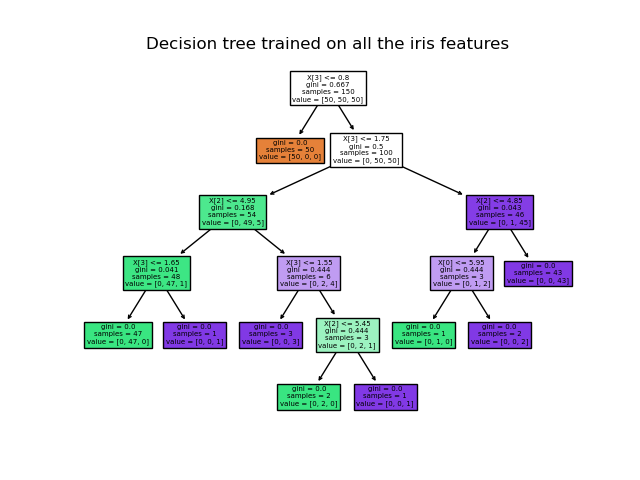
\includegraphics{Datatree}
    
    
    
Chúng ta sử dụng hàm DecisionTreeRegressor() trong sklearn để thực hiện bài toán hồi quy 
    \begin{lstlisting}[language=Python]
    # Import the necessary modules and libraries
    import numpy as np
    from sklearn.tree import DecisionTreeRegressor
    import matplotlib.pyplot as plt
    
    # Create a random dataset
    rng = np.random.RandomState(1)
    X = np.sort(5 * rng.rand(80, 1), axis=0)
    y = np.sin(X).ravel()
    y[::5] += 3 * (0.5 - rng.rand(16))
    
    # Fit regression model
    regr_1 = DecisionTreeRegressor(max_depth=2)
    regr_2 = DecisionTreeRegressor(max_depth=5)
    regr_1.fit(X, y)
    regr_2.fit(X, y)
    
    # Predict
    X_test = np.arange(0.0, 5.0, 0.01)[:, np.newaxis]
    y_1 = regr_1.predict(X_test)
    y_2 = regr_2.predict(X_test)
    
    # Plot the results
    plt.figure()
    plt.scatter(X, y, s=20, edgecolor="black", c="darkorange", label="data")
    plt.plot(X_test, y_1, color="cornflowerblue", label="max_depth=2", linewidth=2)
    plt.plot(X_test, y_2, color="yellowgreen", label="max_depth=5", linewidth=2)
    plt.xlabel("data")
    plt.ylabel("target")
    plt.title("Decision Tree Regression")
    plt.legend()
    plt.show()
    \end{lstlisting}
    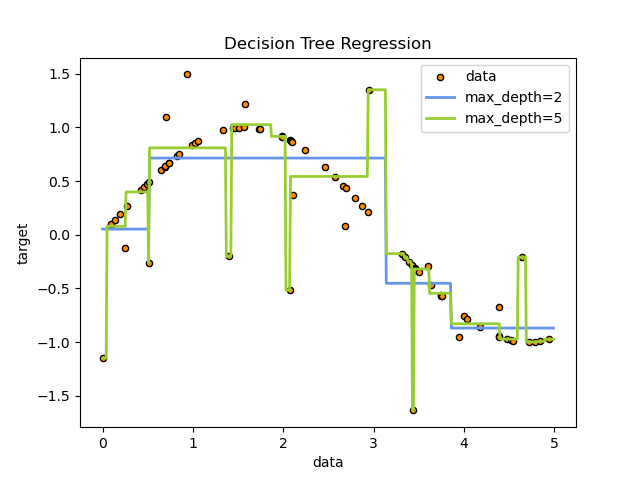
\includegraphics{regression}
\subsection{Các tham số}
Decision tree hỗ trợ rất nhiều tham số mà bạn có thể truyền vào để
tối ưu hóa cây của bạn. Một vài các tham số cần lưu ý như sau:
\begin{itemize}
\item \textbf{criterion}: Tiêu chuẩn tính, bao gồm: \{’gini’, ’entropy’, ’log\_loss’\}.Mặc định là ’gini’. Dùng để xác định tiêu chuẩn chia để tạo decision tree.
\item \textbf{max\_depth}: Nhận vào giá trị là một số nguyên dương, mặc định
là None. Dùng để giới hạn độ sâu của cây. Nếu max\_depth = None
cây sẽ mở rộng đến khi tất cả node lá chứa ít mẫu hơn tham số
min\_samples\_split.
\item \textbf{min\_samples\_split}: Nhận vào giá trị > 0, mặc định là 2. Là số lượng mẫu tối thiểu để tiếp tục tách một node.
\item \textbf{min\_samples\_leaf}: Nhận vào giá trị > 0, mặc định là 1. Là số lượng mẫu tối thiểu cần thiết ở một nút lá.
Việc phân chia một điểm ở bất cứ độ sâu nào chỉ được thực hiện
khi số lượng mẫu phải lón hơn min\_samples\_leaf ở cả nhánh trái
và phải
\item \textbf{max\_leaf\_nodes}: Nhận vào giá trị là một số nguyên dương, mặc
định là None. Trồng cây có số lượng node tối đa theo cách tốt nhât
\end{itemize}
\section{Trình bày thuật toán}
Trước khi trình bày thuật toán ta sẽ đến với hai tiêu chuẩn để chia mục trong Decision Tree đó là Entropy (Shannon entropy) và Gini impurity. Và sau đó là thuật toán ID3. Từ nền tảng toán học đó ta sẽ tiến hành implement Decision Tree
\subsection{Entropy và Information gain }
Entropy là một khái niệm khá thông dụng được dùng trong nhiều lĩnh vực vật lý, toán học v..v.. Trong lĩnh vực xử lý thông tin, nhà toán học Claude Shannon đã đưa ra khái niệm information entropy (Shannon entropy). Shannon entropy thể hiện mức độ hỗn loạn hay độ nhiễu của data. Với một hệ thống với N trạng thái có thể xảy ra thì công thức của Shannon entropy sẽ như ở dưới:
    $$  S= -\sum_{i=1}^N p_i \log_{2} p_i   $$
 
Trong đó  là xác suất trạng thái thứ  xuất hiện ở trong hệ thống. Giá trị entropy càng cao thì độ hỗn loạn của hệ thống càng cao, còn nếu càng thấp thì hệ thống càng có trật tự. Và một hệ thống có trật tự cũng tương đương với việc data được phân nhánh một cách chuẩn chỉ. Vì vậy khi càng có nhiều data, entropy ngày càng có hệ thống hơn và khả năng phân loại ổn định hơn. Do vậy, độ giảm của entropy được gọi là information gain và có công thức như sau:
    $$ IG(Q) = S_0 - \sum_{i=1}^q {\frac{N_i}{N}}S_i   $$ 
    
\begin{itemize}
\item IG : giá trị information gain
\item Q : điều kiện để chia data
\item q : số nhóm sau khi chia
\item $N_i$ : số dữ liệu trong tập
\end{itemize}
\subsection {Gini impurity}
Đơn giản hơn so với Entropy và information gain, Gini Impurity là chỉ số thể hiện mức độ phân loại sai khi ta chọn ngẫu nhiên một phần tử từ tập data. Gini Impurity có công thức như sau:

  $$ G=\sum_{k} p_k * (1-p_k)^2 = 1- \sum_{k} (p_k)^2 $$
 

\begin{itemize}
\item G: giá trị Gini Impurity
\item K: số các lớp có trong tập data
\item $p_k$ :xác suất mà một phần tử ngẫu nhiên thuộc lớp 
\end{itemize}
 Ta thấy, giá trị Gini Impurity sau khi chia của mỗi nhóm đều nhỏ hơn so với giá trị ban đầu => Sau khi chia nhóm mức độ phân loại sai của hệ thống đã giảm. Độ giảm của Gini Impurity được gọi là Gini Gain và có công thức tính tương tự như information gain, chỉ khác là ta sẽ sử dụng giá trị Gini Impurity thay vì Entropy:
    $$ GG(Q)= G_0 - \sum_{i=1}^q \frac{N_i}{N} G_i $$
\subsection {Thuật toán ID3}
ID3 (Iterative Dichotomiser 3) được phát triển vào năm 1986 bởi Ross Quinlan. Thuật toán tạo ra một cây đa đường, tìm cho mỗi nút (Greedy) phân loại nhiều mục,từ đó phân loại tối đa các đặc trưng của mẫu.Cây luôn đạt kích thước tối đa và sau đó bước cắt tỉa (pruning) được áp dụng để khái quát hóa dữ liệu sẽ được dự đoán.Thuật toán sử dụng đệ quy (recursive), tham lam (greedy) và chia để trị (Divide and conquer). Ở đây chúng ta sử dụng tiêu chuẩn Gini hay Entropy đều không thay đổi kết quả chọn nhiều lắm 

\textbf{Các bước tiến hành thuật toán} : 

\begin{itemize}
    \item Thuật toán ID3 bắt đầu với tập hợp ban đầu S là nút gốc (root node)
    \item Sau đó mỗi lần đệ quy tính ra những thành phần không sử dụng của tập S, tính ra entropy hoặc là Information Gain. 
    \item Sau khi tính được, chọn Entropy có giá trị nhỏ nhất (hoặc Information gain là lớn nhất) 
    \item Từ việc chọn ta chia cây ra các nhánh nhỏ hơn quyết định dựa trên entropy, sau đó ta tiếp tục đệ quy trên các nhánh con để xác định tiếp, xác định dựa trên nhiều thuộc tính (attributes) khác của cây 
\end{itemize}

Chính vì đệ quy hết mức nên đối với tập data test ta luôn đạt được độ chính xác 100\% nhưng chỉ là chính xác đối với tập test nhưng rất dễ lệch khi xác định trên tập thật. Để khắc phục điều này ta có thể sử dụng cắt tỉa và điều kiện để tổng quát hóa cây, nhằm tăng độ chính xác với dữ liệu chưa biết 

\textbf{Các điều kiện dừng cây} :
\begin{itemize}
    \item Entropy hoặc Information Gain bằng 0 hoặc nhỏ hơn một giá trị chấp nhận được 
    \item Số lượng node hoặc số lượng nhánh cây đạt tới giới hạn 
    \item Sau khi đạt số lượng node hoặc nhánh cây thì tối ưu lại node của cây để tăng độ chính xác trên tập test 
\end{itemize}
\section{Kết luận} 
Decision Tree là một phương pháp để chọn dữ liệu đơn giản và dễ hiểu, tuy nhiên để có độ chính xác cao thì cần phải tối ưu và điều chỉnh cho phù hợp. 

Tài liệu tham khảo:
\begin{itemize}
    \item \em https://machinelearningcoban.com/2018/01/14/id3/
    \item \em https://en.wikipedia.org/wiki/ID3\_algorithm
    \item \em https://www.oreilly.com/library/view/hands-on-machine-learning/9781491962282/
    \item \em https://scikit-learn.org/stable/modules/classes.html#module-sklearn.tree
    \item \em https://scikit-learn.org/stable/modules/tree.html
\end{itemize}
\textbf{Link colab:} \em https://colab.research.google.com/drive/1rfR7k\_xr1hFMTDriWaNFvhotHdTd\_pji\#scrollTo\=JjTJ5D\-QphlW



\end{document}
\begin{lstlisting}[language=Python]
from __future__ import print_function 
import numpy as np 
import pandas as pd 


class TreeNode(object):
    def __init__(self, ids = None, children = [], entropy = 0, depth = 0):
        self.ids = ids           # index of data in this node
        self.entropy = entropy   # entropy, will fill later
        self.depth = depth       # distance to root node
        self.split_attribute = None # Attribute is 
        chosen, is non-leaf
        self.children = children # list of its child nodes
        self.order = None       # order of values of split_
        self.label = None       # label of node if it is a leaf

    def set_properties(self, split_attribute, order):
        self.split_attribute = split_attribute
        self.order = order

    def set_label(self, label):
        self.label = label

# remove probability  0 
def entropy(freq):
    freq_0 = freq[np.array(freq).nonzero()[0]]
    prob_0 = freq_0/float(freq_0.sum())
    return -np.sum(prob_0*np.log(prob_0))

class DecisionTreeID3(object):
    def __init__(self, max_depth= 10, min_samples_split = 2, min_gain = 1e-4):
        self.root = None
        self.max_depth = max_depth 
        self.min_samples_split = min_samples_split 
        self.Ntrain = 0
        self.min_gain = min_gain
    
    def fit(self, data, target):
        self.Ntrain = data.count()[0]
        self.data = data 
        self.attributes = list(data)
        self.target = target 
        self.labels = target.unique()
        
        ids = range(self.Ntrain)
        self.root = TreeNode(ids = ids, entropy = self._entropy(ids), depth = 0)
        queue = [self.root]
        while queue:
            node = queue.pop()
            if node.depth < self.max_depth or node.entropy < self.min_gain:
                node.children = self._split(node)
                if not node.children: #leaf node
                    self._set_label(node)
                queue += node.children
            else:
                self._set_label(node)
                
    def _entropy(self, ids):
        # calculate entropy of a node with index ids
        if len(ids) == 0: return 0
        ids = [i+1 for i in ids] # panda series index starts from 1
        freq = np.array(self.target[ids].value_counts())
        return entropy(freq)

    def _set_label(self, node):
        # find label for a node if it is a leaf
        # simply chose by major voting 
        target_ids = [i + 1 for i in node.ids]  # target is a series variable
        node.set_label(self.target[target_ids].mode()[0]) # most frequent label
    
    def _split(self, node):
        ids = node.ids 
        best_gain = 0
        best_splits = []
        best_attribute = None
        order = None
        sub_data = self.data.iloc[ids, :]
        for i, att in enumerate(self.attributes):
            values = self.data.iloc[ids, i].unique().tolist()
            if len(values) == 1: continue # entropy = 0
            splits = []
            for val in values: 
                sub_ids = sub_data.index[sub_data[att] == val].tolist()
                splits.append([sub_id-1 for sub_id in sub_ids])
            # don't split if a node has too small number of points
            if min(map(len, splits)) < self.min_samples_split: continue
            # information gain
            HxS= 0
            for split in splits:
                HxS += len(split)*self._entropy(split)/len(ids)
            gain = node.entropy - HxS 
            if gain < self.min_gain: continue # stop if small gain 
            if gain > best_gain:
                best_gain = gain 
                best_splits = splits
                best_attribute = att
                order = values
        node.set_properties(best_attribute, order)
        child_nodes = [TreeNode(ids = split,
                     entropy = self._entropy(split), depth = node.depth + 1) for split in best_splits]
        return child_nodes

    def predict(self, new_data):
        """
        :param new_data: a new dataframe, each row is a datapoint
        :return: predicted labels for each row
        """
        npoints = new_data.count()[0]
        labels = [None]*npoints
        for n in range(npoints):
            x = new_data.iloc[n, :] # one point 
            # start from root and recursively travel if not meet a leaf 
            node = self.root
            while node.children: 
                node = node.children[node.order.index(x[node.split_attribute])]
            labels[n] = node.label
            
        return labels

if __name__ == "__main__":
    df = pd.read_csv('weather.csv', index_col = 0, parse_dates = True)
    X = df.iloc[:, :-1]
    y = df.iloc[:, -1]
    tree = DecisionTreeID3(max_depth = 3, min_samples_split = 2)
    tree.fit(X, y)
    print(tree.predict(X))
\end{lstlisting}